\documentclass[10pt]{article} % For LaTeX2e
\usepackage{tmlr}
% If accepted, instead use the following line for the camera-ready submission:
% \usepackage[accepted]{tmlr}
% To de-anonymize for preprint servers:
% \usepackage[preprint]{tmlr}
\usepackage{amsmath,amssymb}
\usepackage{booktabs}
\usepackage{enumitem}
\usepackage{graphicx}
\usepackage{tikz}
\usetikzlibrary{positioning,arrows}
\usepackage{hyperref}
\usepackage{url}
\hypersetup{hidelinks}

\newcommand{\rsix}{r6.2}
\newcommand{\rfour}{r4.2}

\def\month{07}
\def\year{2026}
\def\openreview{\url{https://openreview.net/forum?id=XXXX}}

\title{What Do Benign-Trained Session Language Models Actually Detect? \\ A Mechanistic Audit on Insider-Threat Benchmarks}

% Author block is hidden automatically while the tmlr package is used
% without the [accepted] or [preprint] options.
\author{\name Anonymous Authors \email anonymous@example.com \\
\addr Anonymous Institution}

\begin{document}

\maketitle

\begin{abstract}
Score-level evaluation cannot reveal \emph{what} an anomaly detector has
learned to detect. We develop a mechanistic audit for anomaly language
models---sparse-autoencoder decomposition of adapter-induced
representation changes, validated by causal interventions against matched
controls and labeled by token-level attribution---and apply it to
Qwen3-8B adapted with QLoRA on benign users only, across two CERT
insider-threat benchmarks. Despite similar scores, the audited detectors
rest on qualitatively different internal evidence. On \rsix{}, whose few
malicious users are profile-distinctive within the benign population, the
causally implicated features are almost entirely profile-bound
($99.8$--$100\%$ of activation mass on simulated psychometric and
organizational tokens), consistent with user-profile novelty; on
\rfour{}, four of five causally selected features instead concentrate on
behavioral session events; and subsampling shows that raw positive count
alone does not explain the difference. What reproduces is the pattern,
not the individual features: literal feature transfer across benchmarks
fails, but each benchmark's profile-versus-behavior evidence type recurs
across SAE initializations and benign-only dictionaries, and in smaller
reruns with a repaired serializer and fresh adapter seeds. The resulting
account---when malicious users are systematically distinguishable from
the benign adaptation population through profile attributes, profile
novelty offers a cheap anomaly shortcut; when that shortcut is
unavailable, behavioral evidence dominates---was specified on CERT and
makes an out-of-setting prediction: on TWOS, with real users, real
psychometrics, and no profile-distinctive malicious minority, the audit
should certify behavioral evidence, and it does. The score-level
consequence is stark: compared only against benign users unseen during
adaptation, day-level ROC-AUC falls from $0.95$ to $0.55$ (\rsix{}) and
from $0.96$ to $0.67$ (\rfour{})---apparent strength is largely a
seen-versus-unseen-user effect---and score-time profile masking
\emph{improves} \rfour{}'s unseen-user discrimination. High
anomaly-ranking performance can thus conceal qualitatively
different---and sometimes identity-proxy---internal evidence; mechanistic
auditing makes the difference visible.
\end{abstract}

\section{Introduction}

Enterprise anomaly detection is usually evaluated as a ranking problem: a model
assigns scores, and the question is whether malicious activity ranks above
benign activity. In high-stakes settings such as insider-threat monitoring, a
score alone answers the wrong question. Two detectors with identical ROC
curves can rest on entirely different evidence---one on anomalous
\emph{behavior}, another on incidental properties of who the malicious users
happen to be---and no amount of score-level evaluation can tell them apart
\citep{chandola2009anomaly,yuan2021deep}. Mechanistic interpretability offers
the missing instrument: if the internal computation that raises an anomaly
score can be localized to sparse, causally validated features, then what the
detector actually detects becomes an empirical question
\citep{olah2020zoom,bricken2023monosemanticity}.

This paper develops that instrument as a \emph{mechanistic audit} and reports
what it finds on the standard insider-threat benchmarks. We adapt Qwen3-8B
\citep{qwen3} with QLoRA \citep{hu2022lora,dettmers2023qlora} on structured
session logs from benign users only, isolate the adapter's token-level effect
as residual-stream deltas, decompose those deltas with top-$k$ sparse
autoencoders \citep{gao2024scaling}, and subject selected feature sets to
causal patching and necessity ablation against matched active controls
\citep{zhang2023best}. Because intervention effects on observational
populations are easily inflated, the audit carries its own validity program:
user-level cluster uncertainty, same-user donor exclusion, held-out-user
discovery/confirmation splits, and SAE-seed stability controls. Finally---and
decisively---token-level attribution asks where the causally implicated
features actually fire in the serialized input.

The audit's findings are a dissociation. On CERT \rsix{}, whose evaluation
population contains four malicious users, the causally implicated features are
almost entirely \emph{profile-bound}, placing essentially all of their
activation mass on static psychometric and organizational tokens rather than
behavioral session events, consistent with user-profile novelty. On CERT \rfour{}, whose population contains
sixty malicious users, the natively rediscovered mechanism is
\emph{behavioral}: four of five top features concentrate on session-event
tokens such as durations. Both mechanisms are causally relevant under our
estimands---\rfour{}'s replicates in direction on held-out users
(feature-level independence; one context individually significant), while
\rsix{}'s held-out replication concentrates on its dominant user---and each
feature family is stable across SAE initializations with no counterpart in
the other benchmark's dictionary. What differs is what the selected features
encode. Because the session model is adapted on benign users only,
malicious-population structure cannot alter adapter training; it can,
however, shape both the SAE dictionary (which is fitted on the evaluation
pool) and which directions the audit selects. We tested the natural
selection-stage hypothesis---small positive populations favor profile-bound
selection---by subsampling \rfour{}'s malicious users within its fixed
dictionary, and found it insufficient: even four-user subsamples select
predominantly behavioral features. Retraining both dictionaries on benign
rows alone reproduces the attribution dissociation, so profile capture does
not require positive-shaped dictionaries either. \rsix{}'s
profile capture is a property of that benchmark's label--profile structure
and its adapter's learned geometry, not of small positive populations in
general.

\begin{figure}[t]
\centering
\resizebox{\textwidth}{!}{%
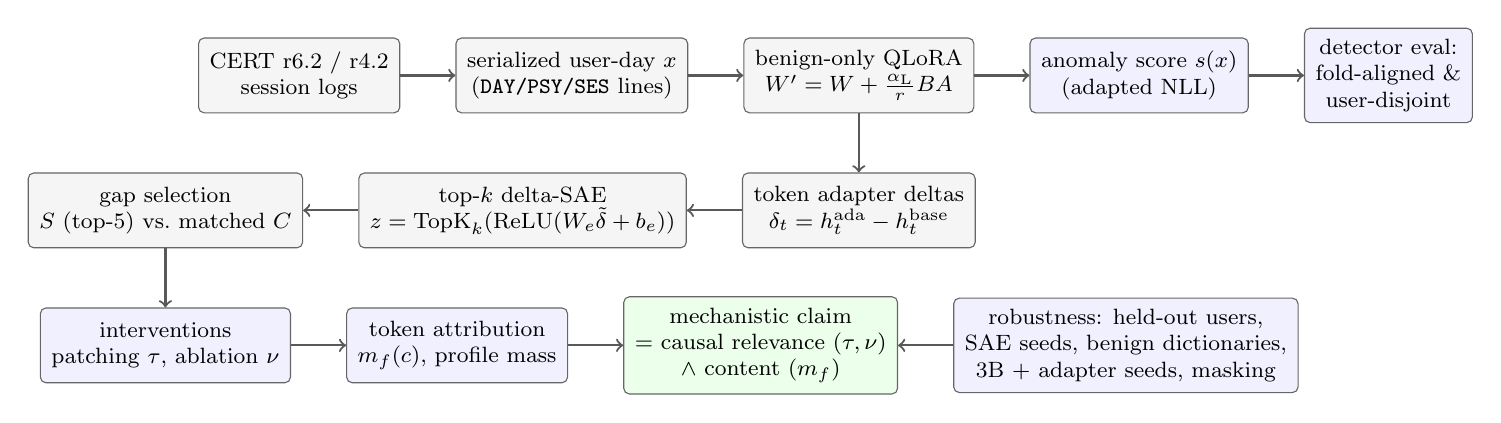
\begin{tikzpicture}[
  box/.style={draw=black!60, rounded corners=2pt, align=center, minimum height=0.95cm, inner sep=4pt, font=\footnotesize},
  stage/.style={box, fill=black!4},
  evalbox/.style={box, fill=blue!6},
  claimbox/.style={box, fill=green!8},
  arrow/.style={->, thick, black!65},
  lab/.style={font=\scriptsize\itshape, black!55}
]
% Row 1: model + score
\node[stage] (data) {CERT \rsix{} / \rfour{}\\session logs};
\node[stage, right=0.7cm of data] (serial) {serialized user-day $x$\\(\texttt{DAY/PSY/SES} lines)};
\node[stage, right=0.7cm of serial] (train) {benign-only QLoRA\\$W' = W + \tfrac{\alpha_{\mathrm{L}}}{r}BA$};
\node[evalbox, right=0.7cm of train] (score) {anomaly score $s(x)$\\(adapted NLL)};
\node[evalbox, right=0.7cm of score] (det) {detector eval:\\fold-aligned \&\\user-disjoint};

% Row 2: mechanism
\node[stage, below=0.75cm of train] (delta) {token adapter deltas\\$\delta_t = h^{\mathrm{ada}}_t - h^{\mathrm{base}}_t$};
\node[stage, left=0.7cm of delta] (sae) {top-$k$ delta-SAE\\$z = \mathrm{TopK}_k(\mathrm{ReLU}(W_e\tilde{\delta}+b_e))$};
\node[stage, left=0.7cm of sae] (select) {gap selection\\$S$ (top-5) vs.\ matched $C$};

% Row 3: audit
\node[evalbox, below=0.75cm of select] (mech) {interventions\\patching $\tau$, ablation $\nu$};
\node[evalbox, right=0.7cm of mech] (attr) {token attribution\\$m_f(c)$, profile mass};
\node[claimbox, right=0.7cm of attr] (claim) {mechanistic claim\\= causal relevance ($\tau,\nu$)\\$\wedge$ content ($m_f$)};
\node[evalbox, right=0.7cm of claim] (robust) {robustness: held-out users,\\SAE seeds, benign dictionaries,\\3B + adapter seeds, masking};

\draw[arrow] (data) -- (serial);
\draw[arrow] (serial) -- (train);
\draw[arrow] (train) -- (score);
\draw[arrow] (score) -- (det);
\draw[arrow] (train) -- (delta);
\draw[arrow] (delta) -- (sae);
\draw[arrow] (sae) -- (select);
\draw[arrow] (select) -- (mech);
\draw[arrow] (mech) -- (attr);
\draw[arrow] (attr) -- (claim);
\draw[arrow] (robust) -- (claim);
\end{tikzpicture}}%
\caption{The audit pipeline, annotated with the notation of
Section~\ref{sec:formal}. Top row (model and score): session logs are
serialized into structured user-day text $x$ and adapt Qwen3-8B on benign
users only; the adapted NLL $s(x)$ is evaluated under both the fold-aligned
and the user-disjoint detector protocols. Middle row (representation):
token-level adapter deltas $\delta_t$ feed a top-$k$ sparse autoencoder,
and features are selected by activation gap against matched active
controls. Bottom row (audit): intervention estimands ($\tau$: patching;
$\nu$: ablation) certify causal relevance, token attribution $m_f(c)$
identifies content, and only their conjunction---stress-tested by the
robustness battery---licenses a mechanistic claim.}
\label{fig:pipeline}
\end{figure}


\paragraph{Contributions.}
\begin{enumerate}[leftmargin=1.3em]
\item We assemble an intervention-based \emph{mechanistic audit} for anomaly
language models---adapter-delta sparse autoencoders, causal patching and
necessity ablation under active controls, cluster-level uncertainty,
dictionary-conditional held-out-user confirmation, seed-stability controls, and token-level feature
attribution---and apply and stress-test the combined audit on two CERT benchmarks.
\item Using the audit, we show that the same architecture and pipeline learns
mechanisms of different \emph{kinds} on related benchmarks: profile-bound
features consistent with user-profile novelty on \rsix{} ($99.8$--$100\%$ of top-feature activation mass on
psychometric and organizational tokens) versus behavioral session features on
\rfour{}---a failure mode invisible to score-level evaluation. The
dissociation is established for these benchmark--adapter instances (one
adaptation run per benchmark); population-level tests reject positive-count
explanations at the selection stage, and benign-only dictionary retraining
rejects dictionary-formation explanations.
\item We show the two mechanisms are stable subspaces of their own models
(cross-seed decoder alignment $0.81$--$0.95$ in residual-stream
coordinates, above dictionary-median null baselines of $0.72$--$0.82$)
while cross-benchmark top-feature alignment sits at or below its null---at
matched depth, the top features align \emph{worse} than typical dictionary
features---showing that SAE initialization instability is unlikely to
explain the observed transfer failure.
\item We document the audit's validity program: why receiver-level
uncertainty, permissive donor matching, and search-then-evaluate selection
each overstate mechanistic evidence, and how cluster bootstraps, same-user
exclusion, and feature-level discovery/confirmation splits repair them.
\end{enumerate}

\section{Related Work}

\paragraph{Insider-threat detection.}
The CERT insider-threat test datasets \citep{glasser2013bridging,certdataset}
are the standard public benchmarks for user-behavior-based insider-threat
detection. Prior work spans unsupervised deep models over aggregated user-day
features \citep{tuor2017deep}, systematic studies of data granularity
\citep{le2020analyzing}, and a broad deep-learning literature reviewed by
\citet{yuan2021deep}. Our baseline detectors follow this tradition: one-class
detectors (Deep SVDD \citep{ruff2018deepsvdd}, GRU and LSTM autoencoders,
Isolation Forest \citep{liu2008isolation}) over session-level behavioral
features. Our contribution is orthogonal to detector engineering: we ask
whether a sequence-native language model trained on the same benign population
admits a causal, feature-level account of its anomaly evidence.

\paragraph{Language models over logs.}
Treating system and behavior logs as sequences for anomaly detection predates
modern LLMs \citep{du2017deeplog,guo2021logbert}. These approaches inherit the
transformer's sequence modeling capacity \citep{vaswani2017attention} but are
typically evaluated only as detectors. We instead use parameter-efficient
adaptation \citep{hu2022lora,dettmers2023qlora} of a general-purpose LLM
\citep{qwen3} and center the evaluation on the internal structure induced by
adaptation rather than on detection leaderboards. This detector class is no
longer hypothetical: LoRA-tuned and LLM-based insider-threat log analysis
systems are actively being developed \citep{song2025dmfi,sun2025redchronos},
which makes auditing what such detectors learn a timely obligation rather
than a retrospective one; to our knowledge, ours is the first end-to-end
causal audit of what an adaptation-based anomaly detector's score rests
on.

\paragraph{Mechanistic interpretability.}
Sparse autoencoders and dictionary learning decompose model activations into
sparse, more interpretable features
\citep{cunningham2023sparse,bricken2023monosemanticity,gao2024scaling}.
Intervention-based validation---activation patching, causal mediation, and
ablation---provides the causal counterpart
\citep{vig2020investigating,meng2022locating,zhang2023best,heimersheim2024use},
with causal scrubbing formalizing hypothesis testing over internal computations
\citep{chan2022causal}. Circuit-level studies have largely targeted curated
natural-language behaviors \citep{wang2023interpretability}. Two design choices
in our protocol follow explicit recommendations from this literature: effects
are always measured against matched active controls rather than in isolation
\citep{zhang2023best}, and we treat cross-dataset transfer of a mechanism as an
empirical claim to be tested rather than assumed, connecting to the question
of universality of learned structure \citep{olah2020zoom,chughtai2023toy}.
Like recent work analyzing LoRA-induced \emph{delta activations} with sparse
autoencoders \citep{prasanth2026lora}, our decomposition targets what
fine-tuning adds to the residual stream rather than raw activations; our
contribution is not the delta-SAE construction itself but its combination
with intervention-based validation under matched controls, user-disjoint
security evaluation, and semantic attribution into an end-to-end audit.

\paragraph{Shortcut learning and evaluation pitfalls.}
Our central finding is an instance of shortcut learning: models satisfying a
training objective through features that do not generalize as intended
\citep{geirhos2020shortcut,lapuschkin2019unmasking}, a risk amplified when
pipelines are underspecified by their evaluations
\citep{damour2020underspecification}. Closest to our setting, the Clever
Hans effect has been demonstrated in anomaly detection specifically, with
explanation methods revealing detectors that rely on spurious input
components \citep{kauffmann2020clever}; our audit extends that program from
attribution over inputs to causally validated sparse features inside an
adapted language model.
In security applications specifically, sampling bias, label artifacts, and
inappropriate train/test separation are documented recurrent pitfalls
\citep{arp2022dos}; our user-disjoint detector analysis and profile-masking
counterfactuals are instances of the evaluation hygiene that work
prescribes. On the interpretability side, SAE feature identity is itself an
unstable object---features can split or absorb one another across dictionary
configurations \citep{chanin2024absorption}---which motivates our seed
controls, matched-layer alignment baselines, and the benign-only dictionary
retraining check.

\section{Benchmarks and Session Modeling}
\label{sec:data}

\paragraph{Datasets.}
We use CERT \rsix{} and \rfour{} \citep{glasser2013bridging,certdataset},
simulated enterprise environments with ground-truth insider incidents.
Following the LC-DAL feature-extraction line used by our baseline detectors, raw
event logs are aggregated into per-session behavioral feature vectors
(logon/logoff structure, file, device, HTTP, and email activity), grouped into
user-days. Each example in our corpus is one user-day.

\paragraph{Evaluation population.}
All results are stated over the \emph{matched active-session} domain: user-days
that appear in the LC-DAL session-feature extraction. This domain is smaller
than the raw answer key, because some labeled incidents fall outside active
session coverage. For \rsix{}, the matched domain contains $70$ positive
user-days across $4$ malicious users (the answer key lists $99$ positive rows
across $5$ users); for \rfour{}, it contains $1309$ positive user-days across
$60$ users (answer key: $1883$ rows across $70$ users). We report this
explicitly because population re-filtering is a common source of silent
optimism in insider-threat evaluation.

\paragraph{Serialization.}
Each user-day is rendered as structured text: a \texttt{DAY} header with
organizational context (week, project, role, business and functional unit,
department, team, IT-administrator flag), a \texttt{PSY} line with the five
simulated psychometric traits, a session-count line, and one \texttt{SES} line
per session listing its numeric LC-DAL features as \texttt{key=value} pairs.
The serialization is deliberately non-prose: the model must learn behavioral
regularities from structured key-value sequences, not natural-language cues.
Four hyphenated file-transfer columns are dropped by the serializer due to a
column-naming constraint (all four exist in \rsix{}'s raw schema;
\rfour{}'s release contains only one of them); we treat the serialized
field set, not the full LC-DAL schema, as the model's observation space.
A smaller-scale rerun with the defect repaired reproduces the paper's
central attribution result (Section~\ref{sec:cross}).

\paragraph{Splits.}
Users with any positive day are assigned entirely to an evaluation split;
benign users are hashed to a validation split with probability $0.10$ and
otherwise to training. Training and early stopping therefore never see
malicious users, making the adapted model a one-class detector at the
population level, not merely at the label level.

\section{Model and Sparse Feature Extraction}
\label{sec:model}

\paragraph{Benign-only adaptation.}
We adapt Qwen3-8B \citep{qwen3} with QLoRA \citep{dettmers2023qlora}: the base
model is quantized to 4-bit NF4 with double quantization and bfloat16 compute,
and low-rank adapters \citep{hu2022lora} with rank $16$, scaling $\alpha=32$,
and dropout $0.05$ are attached to all attention and MLP projection matrices.
Training minimizes next-token negative log-likelihood on benign training
user-days only (sequence length $2048$, effective batch size $8$, one epoch,
learning rate $1.5\times10^{-4}$ with cosine decay and $3\%$ warmup). The
per-example anomaly score is the length-normalized NLL of the serialized
user-day under the adapted model (\emph{adapted NLL}); we also report base-model
NLL and their difference as reference scores.

\paragraph{Token-level adapter deltas.}
For a layer $\ell$, let $h^{\mathrm{ada}}_{t}$ and $h^{\mathrm{base}}_{t}$ be
the residual-stream states of token $t$ under the adapted and base model on the
same input. The \emph{adapter delta} $\delta_t = h^{\mathrm{ada}}_{t} -
h^{\mathrm{base}}_{t}$ isolates what benign-only adaptation changed about the
representation of token $t$. We train top-$k$ sparse autoencoders
\citep{gao2024scaling} on token deltas from the evaluation pool---all
positive-example rows plus subsampled benign rows
(Appendix~\ref{app:methods})---using a ReLU encoder, a top-$k$ mask, and an
untied linear decoder, with latent dimension a multiplier $m$ of the model
width. Because the dictionary is fitted on the full evaluation pool, all
held-out analyses below provide feature-selection and evaluation independence
\emph{conditional on this shared dictionary}, not dictionary-level
independence; we flag this wherever held-out results are claimed. As a
dictionary-independence check, we additionally retrained both SAEs from
scratch on benign rows only---no positive example enters dictionary
formation---and reran selection, attribution, and held-out evaluation
(Section~\ref{sec:cross}): the attribution dissociation reproduces exactly,
while replication of the intervention estimands is partly
dictionary-sensitive. The headline \rsix{} configuration uses layer $18$,
$m=4$, $k=8$; the headline \rfour{} configuration, found by native search
(Section~\ref{sec:r42}), uses layer $26$, $m=2$, $k=4$. Candidate feature sets
are the top-$5$ features ranked by association between feature activity and
positive examples.

\subsection{Formal pipeline}
\label{sec:formal}

We collect the full pipeline---adaptation, scoring, delta extraction, sparse
decomposition, intervention estimands, and attribution---in one place.

\textbf{Benign-only QLoRA.}
Let $p_{\theta_0}$ denote the frozen base model with NF4-quantized weights.
For each adapted linear map $W \in \mathbb{R}^{d_{\mathrm{out}} \times
d_{\mathrm{in}}}$, QLoRA parameterizes
$W' = W + \tfrac{\alpha_{\mathrm{L}}}{r}\,BA$ with
$B \in \mathbb{R}^{d_{\mathrm{out}} \times r}$,
$A \in \mathbb{R}^{r \times d_{\mathrm{in}}}$ ($r{=}16$,
$\alpha_{\mathrm{L}}{=}32$), and only $(A,B)$ are trained on the benign
corpus $\mathcal{D}_{\mathrm{ben}}$ of serialized user-days:
\begin{equation}
\mathcal{L}(\theta) \;=\; -\!\!\sum_{x \in \mathcal{D}_{\mathrm{ben}}}
\sum_{t=1}^{|x|} \log p_{\theta}\!\left(x_t \mid x_{<t}\right).
\end{equation}
No positive example influences $\theta$.

\textbf{Anomaly score.}
For a serialized day $x$, the detector score is the length-normalized
adapted negative log-likelihood
\begin{equation}
s(x) \;=\; -\tfrac{1}{|x|}\textstyle\sum_{t} \log
p_{\theta_{\mathrm{ada}}}\!\left(x_t \mid x_{<t}\right),
\end{equation}
with $s_{\mathrm{base}}$ defined analogously under $\theta_0$; days are
ranked by $s$.

\textbf{Adapter deltas.}
Let $h^{(\ell)}_t(x;\theta) \in \mathbb{R}^{d}$ be the layer-$\ell$
residual-stream state at position $t$. The token-level adapter delta
\begin{equation}
\delta_t(x) \;=\; h^{(\ell)}_t(x;\theta_{\mathrm{ada}}) -
h^{(\ell)}_t(x;\theta_0)
\end{equation}
isolates what adaptation adds to the computation at $(\ell, t)$; it is the
object we decompose.

\textbf{Top-$k$ sparse autoencoder.}
Deltas are standardized per coordinate,
$\tilde{\delta} = (\delta - \mu) \oslash \sigma$, and encoded by
\begin{equation}
z(\tilde{\delta}) \;=\; \mathrm{TopK}_{k}\!\bigl(\mathrm{ReLU}(W_e
\tilde{\delta} + b_e)\bigr) \in \mathbb{R}_{\geq 0}^{m d}, \qquad
\hat{\delta} \;=\; W_d\, z,
\end{equation}
where $\mathrm{TopK}_k$ zeroes all but the $k$ largest pre-activations and
$W_d \in \mathbb{R}^{d \times md}$ is an untied linear decoder trained to
minimize $\mathbb{E}\,\|\tilde{\delta} - \hat{\delta}\|_2^2$. The
residual-stream direction of feature $f$ is $u_f = \sigma \odot
W_d[:,f]$ (all cross-dictionary geometry is computed on normalized $u_f$,
not on raw decoder columns, which live in dictionary-specific standardized
coordinates).

\textbf{Feature selection.}
With row labels $y$ inherited from examples, the selection statistic is the
activation gap $g_f = \mathbb{E}[z_f \mid y{=}1] - \mathbb{E}[z_f \mid
y{=}0]$; the audited set $S$ is the top-5 by $g_f$ and $C$ is a matched
active control set ($|C|=|S|$, activation frequency $\geq 0.002$, low
$|g_f|$; dose-matched variants additionally match activation magnitude and
decoder norm).

\textbf{Causal patching (sufficiency-style).}
For receiver $x$ with codes $\{z_t\}$, feature set $F$, donor day $d$ with
prototype $p_f$ (mean donor code over the donor's $F$-active positions), and
strength $\alpha \in \{0.25, 0.5, 0.75, 1\}$, the counterfactual codes are
\begin{equation}
z'_{t,f} \;=\; (1-\alpha)\, z_{t,f} + \alpha\, p_f
\quad \text{for } f \in F,\; t \in T_F, \qquad
T_F = \{t : \textstyle\sum_{f \in F} z_{t,f} > 0\},
\end{equation}
and the injected residual shift at every token is
$\Delta_t = \bigl(\sigma \odot W_d z'_t + \mu\bigr) - \delta_t$, applied by
forward hook at layer $\ell$ during scoring. Writing $s_F(x; d, \alpha)$ for
the patched score, the recorded per-receiver outcome under donor class
$c \in \{\mathrm{ben}, \mathrm{anom}\}$ is the maximal achievable repair
$\Delta^{F}_{c}(x) = \min_{d \in \mathcal{D}_c(x),\, \alpha}
\bigl[s_F(x; d, \alpha) - s(x)\bigr]$, and the estimand is the paired
difference-in-differences
\begin{equation}
\tau \;=\; \underbrace{\bigl(\overline{\Delta^{S}_{\mathrm{anom}}} -
\overline{\Delta^{S}_{\mathrm{ben}}}\bigr)}_{\mathrm{RA}(S)} \;-\;
\underbrace{\bigl(\overline{\Delta^{C}_{\mathrm{anom}}} -
\overline{\Delta^{C}_{\mathrm{ben}}}\bigr)}_{\mathrm{RA}(C)},
\end{equation}
computed over complete-case receivers with same-user donors excluded;
uncertainty is a user-level cluster bootstrap over malicious users.

\textbf{Necessity ablation.}
Identical machinery with $z'_{t,f} = (1-\alpha) z_{t,f}$ (no donor); with
$e_F(x)$ the resulting score change, the estimand contrasts ablation
dependence across receiver classes and feature sets,
$\nu = \bigl[\overline{e_S(x_{\mathrm{ben}})} -
\overline{e_S(x_{\mathrm{pos}})}\bigr] -
\bigl[\overline{e_C(x_{\mathrm{ben}})} -
\overline{e_C(x_{\mathrm{pos}})}\bigr]$ over context-matched pairs.

\textbf{Token attribution.}
Each position carries a line class $c(t) \in \{\texttt{DAY}, \texttt{PSY},
\texttt{SESCOUNT}, \texttt{SES}\}$ from the serialization schema. The
attribution mass of feature $f$ on class $c$ over positive rows is
\begin{equation}
m_f(c) \;=\;
\frac{\sum_{(x,t)\,:\,c(t)=c} z_{t,f}(x)}{\sum_{(x,t)} z_{t,f}(x)},
\qquad \text{profile mass} \;=\; m_f(\texttt{DAY}) + m_f(\texttt{PSY}).
\end{equation}

\textbf{From interventions to mechanism.}
The audit's inferential contract is the conjunction: $\tau > 0$ and
$\nu > 0$ against matched controls establish that $S$ is \emph{causally
implicated} in the score's anomaly evidence (with the estimand-specific
caveats of Appendix~\ref{app:methods}); the attribution profile
$\{m_f\}_{f \in S}$ establishes \emph{what} $S$ encodes; and only together
do they license mechanistic statements of the form ``the detector's anomaly
evidence rides on profile (or behavioral) content.'' Either component alone
underdetermines the mechanism: interventions certify causal relevance of an
unlabeled subspace, and attribution labels a subspace without certifying
relevance.

\section{Evaluation Protocol}
\label{sec:protocol}

\subsection{Fold-aligned detector benchmark}
\label{sec:detprotocol}

The adapted session LM and the feature-based baselines are compared under an
identical fold construction:
one held-out malicious user per fold, $800$ sampled benign test users per fold
(fixed seed), day-level metrics over all test-user rows, and user-level metrics
after max-aggregation over days. The adapted model is trained once on the
benign population and held fixed across folds; the feature-based baselines
retrain per fold on non-test benign users. This asymmetry matters and we
state it plainly: the session LM's training corpus covers roughly $90\%$ of
benign users, so most sampled benign test users were seen (as benign
sequences) during adaptation, whereas the baselines exclude test users from
training. The bias is not hypothetical: restricting the benign comparison population
to never-trained validation-split users collapses day-level ROC-AUC from
$0.954$ to $0.545$ on \rsix{} and from $0.959$ to $0.668$ on \rfour{}
(user-level: $0.970\!\to\!0.546$ and $0.969\!\to\!0.565$). These paired
values are computed on the full evaluation pool; the fold-aligned values in
Table~\ref{tab:cert_detector} ($0.953$/$0.964$) use the baselines' per-fold
test populations and therefore differ in the last digits. Since malicious
users are unseen by construction, the unseen-versus-unseen comparison is the
fairer test of generalization to unseen users: it removes training-seen
status as an explanation for discrimination, and it shows the fold-aligned
ROC advantage is largely a \emph{seen-versus-unseen-user} effect. (Unseen
malicious users can still differ from unseen benign users in profile as well
as behavior; the masking analysis in Section~\ref{sec:counterfactuals} probes whether
the residual signal is behavioral.) The fold-aligned numbers below follow the local baselines' protocol
for comparability, but should be read with this in mind. Scoring uses the full corpus, and fold masks are
applied only afterward. We adopted this protocol after finding that an earlier
pipeline, which re-filtered an already-filtered score file, silently dropped
the benign validation slice and overstated the session LM's detector
precision; all
detector numbers reported here use the corrected full-population path.

\subsection{Mechanistic estimands}
\label{sec:mechprotocol}

Both estimands operate on \emph{receivers} (positive user-day examples) and
report effects of intervening on a selected sparse feature set $S$ relative to
a matched \emph{active control} set $C$ of equally many features drawn from
those with nontrivial activation support (activation frequency at least
$0.002$). Inert controls make intervention effects look artificially large, so
control activity is a precondition, not an afterthought \citep{zhang2023best}.

\paragraph{Causal patching (sufficiency-style evidence).}
For each receiver we select donor user-days matched on an organizational
context mode (role, department$\times$role, project$\times$role, team, or
department), drawn either from benign users or---as a same-class control---from
other anomalous user-days. At token positions where features in $S$ are
active, we patch the delta-SAE features toward the donor prototype and measure
the resulting change in adapted NLL, keeping each receiver's best donor. Let
$\Delta^{S}_{\mathrm{ben}}$ and $\Delta^{S}_{\mathrm{anom}}$ denote a
receiver's best NLL change under benign and anomalous donors. The
\emph{repair advantage} of $S$ is
$\mathrm{RA}(S) = \overline{\Delta^{S}_{\mathrm{anom}}} -
\overline{\Delta^{S}_{\mathrm{ben}}}$,
and the reported estimand is the paired contrast
$\mathrm{RA}(S) - \mathrm{RA}(C)$ computed over receivers with complete
top/control and benign/anomalous donor values. A positive value means the
selected features carry anomaly-specific repairable structure beyond what
matched control features carry.

\paragraph{Ablation (necessity-style evidence).}
For each positive receiver paired with a context-matched benign receiver, we
ablate the selected features and measure the NLL change on both. The
\emph{necessity advantage} is the paired top-versus-control contrast of
(benign minus positive) ablation effects: positive values mean ablating $S$
disrupts anomaly evidence on positive examples more than on matched benign
examples, and more than ablating $C$ does. Throughout, patching establishes
\emph{repairability}---the selected features carry causally useful
information given the rest of the computation---not literal sufficiency of
the features in isolation, and ablation establishes dependence rather than
strict necessity, since redundant pathways may exist.

\paragraph{Same-user exclusion.}
In both estimands, donors and benign matches from the receiver's own user are
excluded. Without this restriction, patching can ``repair'' an anomalous day by
borrowing the same user's benign signature, which inflates effects for reasons
unrelated to the hypothesized mechanism. An audit of earlier permissive-donor
runs found nontrivial same-user matching rates; all mechanistic results
reported here come from reruns with same-user exclusion enforced and verified.

\paragraph{Uncertainty.}
Point estimates are complete paired contrasts, not differences of marginal
means, which diverge when donor availability is asymmetric. Because multiple
positive days from the same user are not independent, headline confidence
intervals use a \emph{user-level cluster bootstrap} ($10{,}000$ draws with the
malicious user as the resampling unit); we additionally report per-user
estimates and leave-one-user-out effects. Receiver-level (day-level) bootstrap
intervals are narrower and are reported only as supplementary material.
Context modes constitute a small multiplicity surface: we report all audited
context modes rather than selecting a winner, quote per-context intervals
without multiplicity adjustment, and treat cross-context consistency of
sign---not any single best context---as the replication criterion; headline
text names the best context only as an exemplar.

\section{Results}
\label{sec:results}

\subsection{Detection: strong ranking, weak day-level precision}
\label{sec:detresults}

Table~\ref{tab:cert_detector} reports the fold-aligned comparison. The adapted
NLL score ranks strongly: day-level ROC-AUC is $0.953$ on \rsix{} and $0.964$
on \rfour{}, user-level ROC-AUC is $0.97$ on both, and the held-out malicious
user ranks in the top $3.5\%$ of $801$ test users on average (mean rank $24.0$
on \rsix{}, $26.4$ on \rfour{}). Adaptation carries the signal: base-model NLL
achieves day ROC-AUC of only $0.461$ (\rsix{}) and $0.581$ (\rfour{}).
Day-level PR-AUC tells a different story: at extreme base rates
($\sim$$10^{-5}$ positive on \rsix{}) the adapted model reaches only
$0.00075$ on \rsix{} and $0.0134$ on \rfour{}, below Deep SVDD
($0.0115$ and $0.0337$) and the recurrent autoencoders, though above Isolation
Forest on both datasets.

\begin{table}[t]
\caption{Detector comparison on CERT under two protocols. Fold-aligned rows follow the baselines' protocol, in which the session LM (trained once on ~90 percent of benign users) faces mostly training-seen benign test users while baselines exclude test users from training; bold marks the best fold-aligned value per metric (held-out rank: lower is better). The italicized user-disjoint rows restrict the LM's benign comparison population to never-trained validation users and are the fair comparison for the LM: its ranking advantage largely disappears (day ROC 0.953 to 0.545 on r6.2; 0.964 to 0.668 on r4.2), showing the fold-aligned strength is mostly a seen-versus-unseen-user effect. User-disjoint PR values are on a different benign population size and are not comparable to the fold-aligned column.}
\label{tab:cert_detector}
\centering
\footnotesize
\setlength{\tabcolsep}{4.5pt}
\begin{tabular}{llcccc}
\toprule
Dataset & Method & Day PR-AUC & Day ROC-AUC & User PR-AUC & Held-out rank \\
\midrule
r6.2 & Session LM (adapted NLL) & 0.0008 & \textbf{0.953} & 0.054 & \textbf{24.0} \\
 & Deep SVDD & \textbf{0.0115} & 0.628 & \textbf{0.211} & 83.2 \\
 & GRU AE & 0.0057 & 0.766 & 0.081 & 24.8 \\
 & LSTM AE & 0.0021 & 0.768 & 0.057 & 24.2 \\
 & Isolation Forest & 0.0002 & 0.713 & 0.013 & 153.0 \\
 & \emph{Session LM, user-disjoint benign} & 0.0005 & 0.545 & 0.013 & -- \\
\midrule
r4.2 & Session LM (adapted NLL) & 0.0134 & \textbf{0.964} & 0.101 & \textbf{26.4} \\
 & Deep SVDD & \textbf{0.0337} & 0.743 & \textbf{0.382} & 53.4 \\
 & GRU AE & 0.0254 & 0.696 & 0.124 & 86.6 \\
 & LSTM AE & 0.0236 & 0.714 & 0.120 & 92.1 \\
 & Isolation Forest & 0.0003 & 0.715 & 0.008 & 186.4 \\
 & \emph{Session LM, user-disjoint benign} & 0.1023 & 0.668 & 0.521 & -- \\
\bottomrule
\end{tabular}
\end{table}


\begin{figure}[t]
\centering

\includegraphics[width=\textwidth]{figures/detector_dissociation.pdf}
\caption{Score-level results. Left two panels: ranking--precision
dissociation under the fold-aligned protocol; each point is one detector, and
the adapted session LM (blue) attains the highest day-level ROC-AUC on both
benchmarks while remaining mid-pack on day-level PR-AUC (log scale) at
extreme base rates. Right panel: that apparent strength largely disappears
when the benign comparison population is restricted to never-trained users
(day ROC $0.954\!\to\!0.545$ on \rsix{}, $0.959\!\to\!0.668$ on \rfour{};
Section~\ref{sec:detresults})---the paper's central score-level finding.}
\label{fig:detector_dissociation}
\end{figure}

Figure~\ref{fig:detector_dissociation} summarizes the pattern. Combined
with the never-trained-benign sensitivity above, the score-level conclusion
anticipates the mechanistic one: the model's ranking strength is largely user
novelty rather than behavioral discrimination: on \rsix{} almost entirely so,
on \rfour{} with a residual anomaly signal ($0.668$ day ROC against unseen
benigns) whose behavioral character is supported by the feature attribution
rather than by the ROC value itself. Stated plainly: under the
user-disjoint comparison the session LM does \emph{not} outperform the
feature-based baselines: its day ROC ($0.545$/$0.668$) falls at or below
every baseline's fold-aligned value ($0.628$--$0.768$), and the baselines
already exclude test users from training. Within-user day ranking sharpens
the picture. For each malicious user we computed the ROC-AUC of the adapted
NLL over that user's own days (positive versus own-benign; identity held
fixed by construction). The score does carry within-user signal on both
benchmarks: mean within-user AUC $0.669$ ($95\%$ user bootstrap
$[0.619, 0.717]$; $52/60$ users above chance) on \rfour{} and $0.725$
($[0.654, 0.795]$; $4/4$ users, e.g.\ the dominant user at $0.768$) on
\rsix{}. User novelty therefore explains the collapse of \emph{cross-user}
ranking---between-user profile novelty swamps the within-user signal when
users are compared---rather than an absence of within-user behavioral
signal; on \rsix{} the latter is consistent with the secondary behavioral
feature family recovered in Section~\ref{sec:cross}. We therefore treat
detection as background and ask what internal structure the benign-only
adaptation induced.

\subsection{\rsix{}: necessity is consistent across users; causal effects concentrate in one user}
\label{sec:r62}

\begin{figure}[t]
\centering

\includegraphics[width=\textwidth]{figures/mech_effects.pdf}
\caption{Mechanistic effects under same-user exclusion, by benchmark and
estimand (note the panel-specific scales, all in units of $10^{-3}$
adapted-NLL). Points are paired complete-case top-versus-control contrasts;
horizontal lines are $95\%$ user-level cluster bootstrap intervals
($10{,}000$ draws with the malicious user as resampling unit; the prespecified
primary analysis); open markers denote intervals that cross zero. In the
causal panels, the dashed line marks the best matched session-autoencoder
comparator contrast on the same receivers (indicative only; the comparator
operates on a different score scale).}
\label{fig:mech_effects}
\end{figure}

Figure~\ref{fig:mech_effects} shows all headline mechanistic effects.
Because gap-ranked features carry more activation energy than active
controls, the headline contrasts were re-verified against
\emph{dose-matched} controls (features matched on activation frequency,
magnitude, and decoder norm; edit-size gap closed to $1.3$--$1.8\times$;
Appendix~\ref{app:methods}): all four contrasts remain positive, with the
\rfour{} causal contrast ($+0.0017$ $[0.0011, 0.0023]$) and the \rsix{}
necessity contrast ($+0.061$ $[0.007, 0.084]$) individually significant.
\rsix{} patching is the weakest link (positive but descriptive with four
clusters); its causal evidence rests on necessity and the donor-type
contrast.
The $70$ positive receiver-days on \rsix{} come from only four malicious
users, with highly unequal day counts ($46/18/5/1$), so we treat per-user
structure as part of the result rather than pooling days as independent units.
The necessity side is the strongest \rsix{} finding: ablating the layer-18
top-5 features harms anomaly evidence more than ablating matched active
controls for \emph{every} malicious user in the project$\times$role context
(per-user effects $0.019$--$0.103$; pooled $0.065$; cluster interval
$[0.026, 0.083]$, though with only four clusters such intervals are
descriptive rather than conventionally inferential), and the role context is
consistent as well ($0.062$, $[0.016, 0.083]$; three of four users
positive). The causal patching side is positive but concentrated:
the pooled role-context contrast is $0.0068$ with cluster CI
$[0.0001, 0.0100]$, positive for all four users individually, yet dominated by
the most active user ($0.010$ versus $0.0001$--$0.0005$ for the other three),
and the department$\times$role and project$\times$role intervals cross zero
under user-level resampling. The team context yields no finite causal estimate
because same-user exclusion leaves no valid anomalous-donor comparison in that
stratum; we report it as unavailable rather than imputing it.

Two comparisons calibrate these magnitudes. First, the strengthened protocol
matters: same-user exclusion reduced the causal point estimates relative to
earlier permissive-donor runs, so part of the earlier effect was inflated
exactly as the audit hypothesized, but the effect does not vanish. Second, a matched session-autoencoder comparator evaluated on the same
receivers at the same day-level unit yields a best contrast of $0.0011$;
because the comparator's score is on a different scale (autoencoder
reconstruction error rather than NLL), we report this as context rather than
as a ratio, and defer standardized cross-model effect sizes to future work.

Because four users cannot support a split-half confirmation, we ran
leave-one-user-out (LOUO) discovery/confirmation: for each fold, features are
re-selected using only the other three users' positives and effects are
estimated on the held-out user with the configuration frozen. Feature
selection itself proved user-sensitive: the three folds that retain the
dominant user select nearly identical top-5 sets, while the fold that holds
out the dominant user selects a fully disjoint set: \rsix{}'s feature
identity is largely defined by that user's data. The causal effect
nevertheless passes its hardest test: the disjoint features, chosen from the
other users' $24$ days, produce a significant repair effect on the dominant
user's $46$ held-out days ($+0.0037$ to $+0.0038$ across contexts, e.g.
project$\times$role $[0.0020, 0.0056]$), while held-out effects on the
low-activity users are near zero. Held-out necessity is asymmetric: it
replicates on the two multi-day low-activity users (up to $+0.043$,
$[0.030, 0.055]$) but is negative on the dominant-user fold. Causal
repairability therefore transfers to the dominant held-out user while
ablation dependence is user-specific: the SAE space contains multiple
causally effective repair directions discoverable from disjoint user
subsets, but which features a given user's anomaly evidence depends on
varies by user.

\subsection{\rfour{}: direct transfer fails; native rediscovery succeeds}
\label{sec:r42}

Applying the \rsix{} mechanism configuration (layer 18, its SAE, and its
feature sets) directly to \rfour{} produces negative top-versus-control
contrasts across all audited transfer configurations under full uncapped
evaluation on all $1309$ receivers: the best transferred configuration per
sparsity setting reaches $-0.00094$ $[-0.00117, -0.00072]$,
$-0.00105$ $[-0.00149, -0.00064]$, and $-0.00113$ $[-0.00144, -0.00082]$.
Direct transfer of the \rsix{} sparse feature set to \rfour{} thus fails
under every audited configuration: at the level of literal feature identity,
nothing transfers in this training run.

An exploratory search over layers and SAE hyperparameters on \rfour{},
however, identifies a candidate mechanism at layer 26 with a smaller
dictionary ($m=2$, $k=4$). Under same-user exclusion, on populations of
$1039$--$1301$ available receivers from $49$--$54$ malicious users per context
mode, causal contrasts are positive with user-level cluster confidence
intervals excluding zero for all four context modes: team $0.00142$
$[0.00097, 0.00186]$, role $0.00111$ $[0.00064, 0.00154]$,
department$\times$role $0.00107$ $[0.00066, 0.00147]$, and department
$0.00098$ $[0.00058, 0.00136]$; mean-of-user-means intervals also exclude
zero. The session-autoencoder comparator's best day-level contrast on the same
receivers is $0.00091$ (different score scale; context only). Necessity is
positive but partial:
department$\times$role ($0.0029$, $[0.0009, 0.0050]$) and role ($0.0021$,
$[0.0001, 0.0042]$) remain positive under clustering, while department and
team cross zero.

Because this configuration was selected by searching the same positive
population it is evaluated on, we ran a held-out confirmation. The malicious
users were split $30/30$ (by seeded shuffle; $671$ versus $638$ positive
days); features were re-selected using discovery-user positives only---the
resulting top-5 set shares four of five features with the full-population
selection, indicating stable selection across disjoint user subsets---and
effects were then estimated exclusively on the $30$ held-out users with the
configuration frozen. Under the prespecified primary analysis (user-level cluster bootstrap),
all four causal point estimates are positive on held-out users at roughly
half the exploratory magnitude ($0.00034$--$0.00076$)---the expected
signature of selection inflation---but only the department context
individually excludes zero ($0.00076$, cluster CI $[0.00035, 0.00121]$;
$21$ of $29$ users positive). We read this as \emph{directional replication}
with one individually significant context, not as confirmation of all four.
Held-out necessity is directionally positive for department$\times$role and
role, while team is a confirmed null. Two caveats bound the claim: the SAE
configuration (layer, dictionary size, sparsity) was fixed by the earlier
full-population search, so independence holds at the feature level only; and
secondary uncertainty procedures (receiver-level, mean-of-user-means) give
more favorable readings that we report in supplementary material rather than
in the headline.

\begin{table}[t]
\caption{Mechanistic summary (best context mode per estimand). All rows use the same-user-excluded protocol with active-control feature sets; the transferred row applies the r6.2 layer-18 configuration to r4.2 without re-fitting. Effects are paired complete-case top-versus-control contrasts with 95\% bootstrap confidence intervals. Comparator ratios are relative to the best matched session-autoencoder contrast on the same receivers (r6.2: 0.001133; r4.2: 0.000909).}
\label{tab:cert_mechanistic}
\centering
\small
\begin{tabular}{lllccl}
\toprule
Dataset & Estimand & Context & Effect & 95\% CI & Note \\
\midrule
r6.2 & Token-SAE causal & role & 0.006848 & [0.000092, 0.010000] & 4/4 users positive \\
r6.2 & Token-SAE necessity & project$\times$role & 0.065188 & [0.026059, 0.082920] & 4/4 users positive \\
\midrule
r4.2 & Transferred causal & multiple & $<0$ & all audited configs $<0$ & direct transfer fails \\
r4.2 & Native token-SAE causal & team & 0.001418 & [0.000967, 0.001863] & all contexts positive \\
r4.2 & Native token-SAE necessity & dept$\times$role & 0.002922 & [0.000911, 0.005005] & necessity partial \\
\bottomrule
\end{tabular}
\end{table}


\subsection{What the mechanisms encode: profile novelty versus behavior}
\label{sec:attribution}

The estimands above establish that causally relevant sparse structure exists;
they do not say what it represents. We therefore attribute each headline
feature's post-top-$k$ activation mass to the serialization's line classes
(\texttt{DAY} organizational header, \texttt{PSY} psychometrics,
\texttt{SES} behavioral session events) on all positive examples, with a
benign contrast set, normalizing by each class's token share
(Table~\ref{tab:attribution}).

The result is unambiguous and opposite between benchmarks. The benign
contrast sharpens it: on benign examples the same \rsix{} features place
essentially zero mass on \texttt{PSY} tokens (e.g., the top feature:
$0\%$ benign versus $99.8\%$ positive), so profile-token firing is specific
to unfamiliar profiles rather than to psychometric tokens per se. On
\rsix{}, the five top causal features place $99.8$--$100\%$ of their
activation mass on profile tokens---four on the \texttt{PSY} line (enrichment $\approx$$13\times$
over token share; the highest-activating tokens are the psychometric digit
values themselves) and one on the \texttt{DAY} header---while behavioral
\texttt{SES} tokens, $78\%$ of the input, carry $\leq 0.2\%$ of the mass.
The \rsix{} mechanism is \emph{profile-bound}, in a pattern consistent
with user-profile novelty: the benign-only adapter learned the benign
population's profile distribution, and
unseen malicious users' profile fields produce large adapter deltas. This
single fact retroactively explains the \rsix{} phenomenology: causal repair
concentrates in the dominant user (patching profile tokens toward a
context-matched donor makes the profile look familiar), necessity does not
transfer across users (each user's profile is constant), and feature identity
flips when the dominant user leaves the selection set.

On \rfour{}, four of the five top features are \emph{behavioral}: they place
$99.9$--$100\%$ of their mass on \texttt{SES} tokens (enrichment $1.33\times$
over the $75\%$ token share) with essentially zero psychometric mass, and one
fires specifically on session-duration fields; the fifth is
\texttt{DAY}-bound. A natural first hypothesis for the contrast is the malicious population's
structure---with four positive users, identity is the cheapest separator;
with sixty, behavioral regularities carry the evidence---but
Section~\ref{sec:cross} tests this directly and rejects its strong form,
pointing instead to finer benchmark properties.

\begin{table}[t]
\caption{Token attribution of the top-5 causal features (positive examples). Columns are activation-mass fractions by serialization line class; PSY enrich is mass fraction over token share for the psychometric line. r6.2 features are profile-bound; four of five r4.2 features are behavioral (SES enrichment 1.33x over a 0.75 token share).}
\label{tab:attribution}
\centering
\footnotesize
\setlength{\tabcolsep}{4.5pt}
\begin{tabular}{llccccl}
\toprule
Bench & Feature & PSY mass & DAY mass & SES mass & PSY enrich & Top tokens \\
\midrule
r6.2 & 14358 & 0.998 & 0.000 & 0.002 & 13.4$\times$ & psychometric values \\
r6.2 & 12848 & 0.999 & 0.000 & 0.001 & 13.4$\times$ & psychometric values \\
r6.2 & 4196 & 1.000 & 0.000 & 0.000 & 13.4$\times$ & psychometric values \\
r6.2 & 13580 & 0.000 & 0.999 & 0.001 & $\approx$0 & org header \\
r6.2 & 11292 & 1.000 & 0.000 & 0.000 & 13.4$\times$ & psychometric values \\
\midrule
r4.2 & 4596 & 0.001 & 0.000 & 0.999 & $\approx$0 & session values \\
r4.2 & 3673 & 0.000 & 0.000 & 1.000 & $\approx$0 & session durations \\
r4.2 & 2302 & 0.001 & 0.998 & 0.001 & $\approx$0 & org header \\
r4.2 & 3455 & 0.000 & 0.000 & 1.000 & $\approx$0 & session values \\
r4.2 & 1268 & 0.000 & 0.000 & 1.000 & $\approx$0 & session values \\
\bottomrule
\end{tabular}
\end{table}


\subsection{Seed-stability controls: the dissociation is not dictionary noise}
\label{sec:seeds}

Sparse dictionaries are not identifiable: literal feature coordinates can fail
to transfer even between two SAE seeds on the same data, so cross-benchmark
transfer failure could in principle say nothing about benchmarks. We retrained
the headline SAE configuration with two fresh seeds per benchmark on the same
cached deltas. Because every SAE decodes into the same $d_{\mathrm{model}}$
residual space, feature correspondence is measurable as decoder cosine
similarity (Table~\ref{tab:alignment}): within a benchmark, each seed's top-5
features have close counterparts in every other seed's dictionary
($|\cos|$ $0.81$--$0.95$ against empirical dictionary-wide best-match
dictionary-median null baselines of $0.72$--$0.82$); across benchmarks,
top-5 best matches sit at or below their nulls ($0.22$--$0.24$ against
nulls of $0.22$--$0.40$ at native layers) in both directions. All geometry
is computed in original residual-stream coordinates: decoder columns are
mapped back through each SAE's per-coordinate standardization scale before
normalization, since raw standardized columns from dictionaries with
different scales are not mutually comparable (the raw-coordinate
comparison, our earlier convention, gives the same qualitative pattern).
Causal rediscovery is likewise seed-robust: fresh-seed SAEs with their own
re-selected features reproduce positive \rsix{} contrasts in every finite
context (e.g., role $0.0071$ and $0.0019$ under seeds 43 and 44, versus
$0.0068$ originally). The profile-bound and behavioral feature families are each stable across
SAE initializations for the same cached adapter representations
(adapter-seed robustness remains untested); their non-correspondence across
benchmarks is a property of the benchmark--adapter pairs. The native-layer
cross-benchmark comparison (18 versus 26) sits at or below the empirical
null, but that partly reflects a depth difference. The matched-layer
comparison at layer 18 is sharper: overall dictionary geometry is
substantially shared there (whole-dictionary median best-match up to
$0.96$, as expected since both SAEs encode the same base model's layer-18
residual stream), yet the \emph{top-5} features align at or below those
medians ($0.30$ and $0.65$): the anomaly-relevant directions are more
benchmark-specific than typical dictionary directions. Matched-layer top-5
alignment also remains below within-benchmark cross-seed alignment
($0.81$--$0.95$), so the distinct headline mechanisms are not consistent
with a simple feature relabeling of one shared sparse representation, even
after controlling for depth. (r4.2's headline mechanism is itself at layer 26;
its layer-18 features used here are off-mechanism, which further limits the
correspondence one should expect.)

\begin{table}[t]
\caption{Feature alignment in residual-stream coordinates (decoder columns mapped back through each SAE's per-coordinate standardization before normalization). Best-match $|\cos|$ of each source SAE's top-5 features into a target dictionary, versus the whole-dictionary median (empirical null). Within-benchmark cross-seed alignment exceeds the null; cross-benchmark top-5 alignment sits at or below its null---at matched layer the top features align worse than typical dictionary features despite substantially shared overall geometry.}
\label{tab:alignment}
\centering
\small
\begin{tabular}{lcc}
\toprule
Comparison & Top-5 best-match $|\cos|$ & Empirical null baseline \\
\midrule
within r6.2 (3 seed pairs) & 0.807--0.856 & 0.720--0.750 \\
within r4.2 (3 seed pairs) & 0.837--0.946 & 0.814--0.818 \\
across benchmarks, native layers (18 vs 26) & 0.218--0.236 & 0.224--0.405 \\
across benchmarks, matched layer 18 & 0.295--0.652 & 0.370--0.963 \\
\bottomrule
\end{tabular}
\end{table}


\subsection{Dictionary and population robustness}
\label{sec:cross}

The picture so far (Table~\ref{tab:claim_status}): benign-only adaptation
induces sparse token-level structure that is causally implicated in anomaly
evidence on both benchmarks, with held-out replication that is directional
on \rfour{} and dominant-user-concentrated on \rsix{}; the structure is
benchmark-specific not merely in coordinates but in \emph{kind}: identity
metadata on \rsix{}, behavior on \rfour{}. This subsection stress-tests
that picture against the two remaining artifact explanations: the positive
population and the dictionary. We tested the population-size hypothesis directly by malicious-population
subsampling on \rfour{}: holding the model, benchmark, SAE dictionary, and
benign population fixed, we resampled positive populations of
$K=4,10,20,30,60$ users (ten repetitions each) and re-ranked features for
each. The strong form of the hypothesis is \emph{rejected at the
feature-selection stage}: profile-mass share among top-5 features
is nearly flat in $K$ ($0.25$ at $K{=}4$ versus $0.16$--$0.20$ at
$K\geq 10$; typically one profile-bound feature in five at every size),
nowhere near \rsix{}'s near-total profile dominance. Small malicious
populations tilt selection toward profile features only mildly. Because the
shared dictionary was itself fitted on the full positive population, this
experiment isolates the selection stage conditional on the fixed \rfour{}
dictionary; it does not test whether positive-population size could influence
dictionary formation itself. A stronger check removes positives from
dictionary formation altogether: we retrained both SAEs from scratch on
benign token deltas only and reran the full downstream pipeline: feature
reselection under held-out discipline (discovery users on \rfour{}; LOUO on
\rsix{}), token attribution, and confirmation evaluation. The dissociation
reproduces at the dictionary level. On \rfour{}, the benign-dictionary top-5
places $\geq 94\%$ of activation mass on behavioral \texttt{SES} tokens
(four of five features at $100\%$, profile mass $\approx 0$); on \rsix{},
every LOUO fold's top-5 is $\geq 99\%$ profile-bound, three of four folds
select an identical feature set, and the fold excluding the dominant user
diverges wholesale, mirroring the original dictionary's
dominant-user-defined feature identity
(Table~\ref{tab:dict_robustness}). Held-out intervention effects are
estimand-dependent under the new dictionaries: \rfour{} necessity replicates
across all four contexts ($+0.004$ to $+0.013$; $528$--$638$ complete pairs),
while its patch-repair contrast does not ($-0.0002$ to $-0.0004$); on
\rsix{}, causal repair is positive on one held-out fold and necessity on the
dominant-user fold. What the selected features \emph{encode} is therefore
dictionary-independent; which intervention estimand replicates on which
held-out users is not (Table~\ref{tab:dict_robustness}). \rsix{}'s
profile capture therefore reflects benchmark-specific factors---plausibly the
distinctiveness of its four malicious users' profile fields within its benign
profile distribution, and properties of its adapter's learned geometry---and
identifying which benchmark properties drive metadata capture is an open
question the audit makes precise.

\begin{table}[t]
\caption{Dictionary-independence summary. Attribution (what the selected features encode) reproduces exactly under SAE dictionaries retrained on benign rows only, while held-out replication of the intervention estimands is estimand- and dictionary-dependent.}
\label{tab:dict_robustness}
\centering
\footnotesize
\begin{tabular}{llp{3.4cm}p{3.6cm}p{3.6cm}}
\toprule
Dataset & Dictionary & Attribution & Held-out patching & Held-out ablation \\
\midrule
r6.2 & Full-pool & Profile-bound (99.8--100\%) & Dominant-user concentrated & User-specific (negative on dominant fold) \\
r6.2 & Benign-only & $\geq$99\% profile-bound, all folds & Positive on one held-out fold & Positive on dominant-user fold \\
\midrule
r4.2 & Full-pool & 4/5 behavioral & Directional; one context significant & Partial \\
r4.2 & Benign-only & $\geq$94\% behavioral & Does not replicate & Replicates in all four contexts \\
\bottomrule
\end{tabular}
\end{table}


Finally, a smaller-scale rerun tests scale-, serializer-, and
adapter-seed-dependence jointly. We repaired the serializer defect
(restoring the four omitted file-routing fields on \rsix{}; \rfour{}'s
release contains one of the four), retrained Qwen2.5-3B QLoRA adapters from
scratch with two adapter seeds per benchmark (one epoch; full $287{,}827$-day
corpus on \rfour{}, $300$k of $1.25$M days on \rsix{}), extracted fresh
token deltas at layers $12/18/24$, retrained benign-only dictionaries, and
reran selection and attribution. The dissociation reproduces under both
adapter seeds. On \rfour{}, the selected features are behavioral in every
audited configuration (five of five features $\geq 0.94$ SES mass at the
best layer under both seeds), and the adapters retain unseen-user
discrimination (day ROC $0.678$/$0.718$ against never-trained benigns,
versus $0.668$ at 8B). On \rsix{}, profile-bound features dominate at the
deepest extracted layer under both seeds (three of five and four of five
features at $\approx 100\%$ profile mass), while shallower layers lean
behavioral: at this scale, profile capture concentrates at depth. The two
\rsix{} adapters differ in quality (day ROC $0.414$ versus $0.738$), and
profile dominance is strongest in the better-trained seed, consistent with
profile capture being acquired through adaptation rather than induced by
the serialization defect or particular to the 8B run. Rerunning the
headline intervention estimands on all four 3B adapters replicates the
estimand asymmetry observed under the 8B benign dictionaries: \rfour{}
necessity-style dependence replicates across both adapter seeds with nearly
identical effects ($+0.00218$ and $+0.00215$; $1301$ complete pairs each)
while its patch-repair contrast does not ($-0.0004$ under both seeds), and
\rsix{}'s intervention effects remain seed- and estimand-idiosyncratic
(causal $+0.0175$ under one seed, near zero under the other). Ablation
dependence is thus the seed-robust causal signature of the behavioral
family.

Excluding profile-dominated features from selection likewise reveals that
\rsix{} also contains a \emph{behavioral} feature family: SES-restricted
ranking under LOUO discipline selects stable behavioral features (two of the
top five recur across three of four folds, all with near-zero profile mass),
and these features carry held-out causal effect on the dominant user
($+0.0027$ to $+0.0029$ across contexts, roughly three-quarters of the
profile-feature effect), with partial held-out necessity (positive on the
small multi-day users; role-context positive on the dominant-user fold, where
the profile features' necessity was uniformly negative). \rsix{}'s profile
capture is therefore a property of unconstrained feature \emph{selection},
not an absence of behavioral causal structure, which is precisely the kind
of distinction the audit exists to make.

\subsection{Score-level profile counterfactuals}
\label{sec:counterfactuals}

A score-time ablation asks what the \emph{score} is sensitive to. We re-serialized the
evaluation population without the \texttt{PSY} line (\emph{no-psy}) and
additionally with organizational identifiers masked (\emph{no-profile}), and
rescored with the frozen models on a fixed unseen-versus-unseen rescoring
population: all positive user-days plus every never-trained benign user
(on \rfour{}: $89$ benign users---the $79$ validation-split users plus $10$
never-trained others---for $42{,}468$ day rows from $149$ users), which is
why the original-arm values here differ slightly from the val-only analysis
of Section~\ref{sec:detresults} (day ROC $0.670$ versus $0.668$; user ROC
$0.666$ versus $0.565$, the latter sensitive to the ten added users under
max-aggregation). Uncertainty for the masking contrasts uses the same
user-level cluster bootstrap as the mechanistic estimands ($10{,}000$ draws,
users as resampling units stratified by label, paired within draws). On
\rsix{}, all three variants remain near chance at the day level (ROC $0.547$
original, $0.575$ no-psy, $0.471$ no-profile) and no masking change is
significant (all $\Delta$ROC intervals span zero; descriptive with four
malicious clusters): with every user unseen, profile novelty separates
nothing, and no clear behavioral signal is revealed underneath. On \rfour{}, masking
psychometrics \emph{improves} discrimination substantially (day ROC
$0.670\!\to\!0.797$, $\Delta$ROC $+0.127$ $[0.061, 0.193]$; day PR
$0.069\!\to\!0.112$; user ROC $0.666\!\to\!0.775$, $\Delta$ROC
$+0.108$ $[0.038, 0.179]$; masking all organizational identifiers as well
yields a smaller, nonsignificant day-level gain of $+0.063$
$[-0.003, 0.130]$): the simulated psychometric fields were not merely
uninformative but actively obscured behavioral signal. Static profile
metadata in the serialization is thus a liability twice over: it invites
identity capture during selection and degrades behavior-based scoring even
when the mechanism is behavioral.


A swap-counterfactual experiment sharpens what the score itself is sensitive
to. For every positive user-day we constructed two variants---profile fields
replaced by a random benign (validation-split) user's, and conversely the
entire behavioral content replaced while keeping the profile---and rescored
with the frozen models. On \emph{both} benchmarks, the score is more
disturbed by profile perturbation than by replacing all behavior
(mean $\Delta$NLL $+0.155$ versus $+0.072$ on \rsix{}, ratio $2.2$;
$+0.180$ versus $+0.102$ on \rfour{}, ratio $1.8$). Because donors are
unseen users, this measures perturbation sensitivity rather than profile
familiarity, and it shows that profile tokens dominate the raw NLL surface of
both adapters, consistent with masking \emph{improving} \rfour{}
discrimination by removing profile-driven score variance. The benchmarks thus
differ not in raw score sensitivity, which is profile-dominated everywhere,
but in where the anomaly-\emph{discriminative} signal lives: a distinction
that feature-level attribution and masking expose and that score-level
perturbation alone cannot.
\subsection{Real-data replication with real psychometrics (TWOS)}
\label{sec:twos}

All results above are on simulated CERT data, and the population-structure
account makes a falsifiable prediction about real data: when malicious users
are \emph{not} a small distinctive minority, identity is a poor separator
and selection should be behavioral. TWOS \citep{harilal2017twos} provides
exactly this test: $24$ real users over five days, staged masquerade
sessions on $12$ of them ($50\%$ prevalence), and---critically---each
user's \emph{real} IPIP-50 Big-Five inventory, giving a genuine
psychometric \texttt{PSY} line where CERT's is simulated. We serialized
mouse, keystroke, and login telemetry into CERT-analogous ten-minute
windows ($18{,}048$ windows; $138$ positive; $12$-user benign train pool),
ran the identical pipeline at smaller scale (Qwen2.5-3B benign-only QLoRA,
two adapter seeds; benign-only dictionaries; full-pool selection;
attribution), and reran the headline intervention estimands.

The audit certifies a clean detector on this benchmark: top-5 attribution
is essentially $100\%$ behavioral under both adapter seeds at both audited
layers (worst single feature: $0.983$ SES mass), despite real personality
scores being present in every window; the score carries real signal
(mean within-user ROC $0.783$ across the $16$ malicious users, identity
held fixed by construction); and the intervention estimands reproduce the
estimand asymmetry a fourth time (ablation dependence $+0.0019$,
patch-repair $-0.0018$; $138$ receivers, team-matched donors, same-user
excluded). This is the predicted outcome for the high-prevalence corner,
and it complements the \rsix{} corner (four highly distinctive users among
thousands) where profile capture wins: the dissociation's behavioral pole
is not an artifact of synthetic data or simulated psychometrics. Deeper
analyses of this benchmark (insider-type boundaries, detector baselines,
per-user failure cases) are developed in companion work.

\begin{table}[htbp]
\caption{Audit claim map: what the evidence supports, rejects, and fails to support.}
\label{tab:claim_status}
\centering
\small
\begin{tabular}{p{7.6cm}p{5.6cm}}
\toprule
Claim & Status \\
\midrule
Benign-only QLoRA training is valid one-class training & Supported \\
Fold-aligned detector strength reflects behavioral discrimination & Rejected (seen-vs-unseen-user effect) \\
r6.2 contains a sparse feature family active on profile tokens whose edits pass the audited estimands & Supported descriptively (best-candidate patching and necessity); held-out replication concentrates on the dominant user; necessity significant against proxy-matched controls (methods appendix) \\
r4.2 contains a sparse feature family active mainly on behavior tokens whose edits pass patching and ablation & Partly: the best-candidate patch contrast is positive (significant against proxy-matched controls), but on held-out users the mean over donors is negative; ablation replication persists under a benign-only dictionary and across 3B adapter seeds, patch-repair replication does not \\
Editing the selected r4.2 features changes behavior-token predictions more than editing controls & Supported for the joint edit under the SAE replacement procedure at strengths 0.75--1 on held-out users; not shown to exceed an equal-size perturbation at the same positions, or to be specific to anomalous days \\
The selected r4.2 edits act on behavior but not profile predictions & Not established: the profile effect is uncertain and the preregistered direct comparison is inconclusive \\
Editing features toward a benign colleague repairs malicious days & Not established: only the searched best candidate is positive; the mean over donors has the opposite sign \\
Configuration-independent r4.2 confirmation & Not established \\
Literal feature transfer across benchmarks succeeds & Rejected \\
Transfer failure is explained by SAE seed non-identifiability & Rejected (alignment controls) \\
Positive-population size alone explains the feature-selection dissociation (conditional on the fixed r4.2 dictionary) & Rejected at the selection stage (subsampling) \\
The profile/behavior attribution dissociation requires positive-shaped dictionaries & Rejected: benign-only SAE retrain reproduces it (r4.2 top-5 $\geq$94\% behavioral; r6.2 $\geq$99\% profile-bound in all LOUO folds) \\
The dissociation is particular to the 8B run, the serializer defect, or one adapter seed & Rejected: 3B repaired-serializer rerun reproduces attribution across two adapter seeds per benchmark, and r4.2 ablation dependence replicates across 3B seeds \\
The behavioral pole is an artifact of synthetic data or simulated psychometrics & Rejected: TWOS (real users, real Big-Five) yields ~100\% behavioral attribution across two adapter seeds at 50\% malicious prevalence, as the population account predicts \\
Profile capture is a generic dataset property that any detector class inherits & Rejected at attribution level: classical one-class detectors on the same r6.2 features place 4--7\% importance on profile, select no profile feature in any top-5, and lose nothing when profile is removed \\
The shortcut is an artifact of CERT's injected profile & Not tested cleanly (corrected 2026-09-24): on LANL, user sampling and fold assignment shared a hash, so the unseen pool is 23 red-team users with no negative-only user and the seen pool adds 988 negative-only users; the AUCs ($0.95$ seen, $0.50$ unseen; host-anonymized $0.88$, $0.63$) describe those pools only; a corrected split is pending \\
Profile content is merely correlated with the unseen-user collapse & Rejected in the audited 8B run: removing profile content from adaptation and scoring restores fold-aligned unseen-user ROC $0.53\to0.90$ (descriptive paired bootstrap interval excluding zero); small and non-significant in the audited 3B run (one adapter seed per arm) \\
\bottomrule
\end{tabular}
\end{table}


\section{Discussion}
\label{sec:discussion}

\paragraph{Audits, not leaderboards.}
Every component of this audit was necessary to reach the finding. Score-level
evaluation showed strong ROC on both benchmarks; the intervention estimands
established causal relevance under at least one audited estimand on both;
the confirmation splits showed
directional held-out replication; the seed controls showed stability across
SAE initializations. Only token-level attribution revealed that one of
them scores evidence consistent with \emph{who a user is} rather than
\emph{what they did}. Any prefix of the audit
would have licensed a stronger---and wrong---behavioral interpretation. We
take this as the central methodological lesson: for anomaly models trained on
metadata-rich telemetry, causal validation and semantic attribution are
separate obligations, and only their conjunction says what a detector
detects. In this sense the audit's mechanistic layer is demonstrably
necessary---every cheaper prefix misleads, and on \rsix{} the black-box
probes were silent where attribution was decisive---while never sufficient
alone: only conjoined with causal validation and score-level evaluation
does it identify what a detector detects. One might object that we audit a
detector of our own construction; but benign-only adaptation is the natural
one-class recipe for the LoRA-tuned insider-detection systems now appearing
\citep{song2025dmfi}, and the failure modes exposed here are properties of
metadata-rich serialization and of evaluation protocol---both inherited
from existing practice---rather than of any particular adapter
architecture. A cross-architecture probe sharpens this: classical
one-class detectors (Isolation Forest, one-class SVM, PCA reconstruction)
trained on the same \rsix{} day-level features \emph{with profile columns
included} place only $4$--$7\%$ of permutation-importance mass on profile
fields, select no profile feature in any top-5, and lose nothing when
profile columns are removed. The profile shortcut is therefore not a
generic dataset property inherited by any detector: it emerges in the
sequence-likelihood pathway, where per-user-constant profile tokens are
exactly what a next-token objective is incentivized to compress. The
detector class the field is now adopting carries a shortcut risk its
classical predecessors demonstrably did not---which is why auditing it
matters. Auditing the class before it is deployed is the point.

\paragraph{A failure mode without a simple boundary condition.}
The profile-novelty mechanism is not a bug in the model; it is a solution to
\rsix{}'s separation problem. But the obvious explanation---population
size---fails our direct test at the feature-selection stage: four-user
subsamples of \rfour{} still select
behavioral features. Whatever drives metadata capture on \rsix{} involves
finer benchmark properties (how distinctive the malicious users' profile
fields are within the benign profile distribution; what the benign-only
adapter happened to compress into its deltas)---and, per the
cross-architecture probe, properties of the sequence-likelihood pathway
specifically, since classical detectors on the same features do not take
the shortcut. The account's two corners
are now both instantiated: profile capture where a tiny distinctive
malicious minority makes identity cheap (\rsix{}), and cleanly behavioral
selection where half the population is malicious and identity separates
nothing (TWOS, on real users with real psychometrics;
Section~\ref{sec:twos}). For benchmark design the
implication is in one way stronger: exposing static per-user metadata,
especially simulated psychometrics with no operational counterpart, creates a
capture risk that cannot be predicted from population size and that
score-level evaluation will not notice---it must be audited for. For
deployment, the implication is unchanged and sharp: an identity-proxy
detector generalizes to \emph{new users being unusual}, not to insider
behavior.

\paragraph{Benchmark-specificity, revisited.}
Cross-benchmark transfer of literal features fails while native rediscovery
succeeds on both sides, and the seed controls locate the failure in the
benchmarks rather than in dictionary randomness. The universality question
familiar from interpretability \citep{olah2020zoom,chughtai2023toy} thus
reappears here with a mechanistic finding: we find no evidence that the two
benchmark-specific adapters implement their anomaly signals through directly
corresponding sparse feature families; indeed, the selected evidence differs
in \emph{kind}. What transfers is the audit itself---the pipeline that
finds, validates, and identifies mechanisms---not the mechanisms.

\paragraph{Why the strengthened protocol is load-bearing.}
Four protocol elements changed conclusions materially during this work:
full-population scoring (an earlier re-filtering bug overstated detector
precision), same-user donor exclusion (permissive matching inflated causal
effects), user-level cluster uncertainty and discovery/confirmation splits
(receiver-level intervals and search-then-evaluate selection overstated
significance), and token-level attribution (without it, the profile mechanism
reads as behavioral). None are exotic; all are easy to omit silently. We
report them as part of the contribution because intervention-based
interpretability applied to security data inherits both the pitfalls of
interpretability \citep{heimersheim2024use} and the base-rate pathologies of
anomaly detection \citep{chandola2009anomaly}.

\section{Limitations}
\label{sec:limitations}

Our evaluation population is the matched active-session domain, not the full
CERT answer key; incidents outside session coverage are invisible to all
compared methods. The CERT benchmarks are simulations, and the psychometric and
organizational fields they expose have no real-world measurement counterpart;
results may not transfer to operational telemetry. The serializer omits four file-\emph{routing} sub-count fields
(to-USB, from-USB, file-activity-type, and disk transfer counts) due to a
column-naming constraint, while retaining the principal behavioral signals:
total USB events and mean USB session duration, total and executable file
counts, e-mail volumes and attachment statistics, off-hours and weekend
flags, session durations, and HTTP category counts including leak- and
hacking-site visits. Claims about the mechanism concern this serialized field
set; the repaired-serializer rerun (Section~\ref{sec:cross}) shows the
attribution dissociation does not depend on the omission. Day-level PR-AUC of the adapted session LM
is weak in absolute terms at realistic base rates. \rsix{} mechanistic
estimates rest on $70$ receivers from $4$ malicious users with highly unequal
day counts, so its causal effect is dominated by a single user and one context
mode (team) is unavailable under strict donor rules; we report cluster
intervals, per-user effects, and leave-one-user-out results for this reason.
The \rfour{} native configuration was found by search, so we report a
dictionary-conditional held-out-user confirmation alongside the exploratory estimates; the confirmed
effect sizes are roughly half the exploratory ones, and only the department
context is individually significant under the strictest user-level resampling.
For \rsix{}, the analogous leave-one-user-out confirmation recovers a
significant held-out causal effect on the dominant user but near-zero causal
effects on the low-activity users, and held-out necessity does not transfer
to the dominant user; \rsix{} claims should be read at that resolution. All mechanistic results
concern feature-level interventions at a single layer under a specific SAE
family; they localize causal structure but do not constitute a complete
circuit-level account \citep{chan2022causal}. Attribution is based on activation mass over line classes; it identifies
where features fire rather than fully specifying their computation, and the
masking and swap experiments of Section~\ref{sec:counterfactuals} provide score-level
profile-sensitivity evidence without identifying individual feature
semantics. The SAE dictionaries were fitted on the full evaluation pool
(including positive rows), so most held-out analyses are
dictionary-conditional; the benign-only retraining check
(Section~\ref{sec:cross}) establishes that the attribution dissociation and
\rfour{}'s necessity-style replication are dictionary-independent, while
patch-repair replication on held-out users is dictionary-sensitive and
should be read as configuration-specific. SAE-seed robustness is established
(Section~\ref{sec:seeds}); the smaller-scale rerun adds attribution-level
replication across two adapter seeds per benchmark and a repaired
serializer, and the headline intervention estimands rerun on the four 3B
adapters replicate \rfour{}'s ablation dependence across seeds; still, the
8B intervention estimands rest on one adaptation run per benchmark and the
rerun's \rsix{} arms train on a capped corpus, so the 8B causal claims
remain scoped to their runs. Relatedly, the
discovery/confirmation splits reselect feature identities but inherit
configuration choices (layer, dictionary size, sparsity, context menu,
intervention grid) made on the full population; confirmation is
feature-level, not configuration-level. Finally, the population-structure explanation for
the profile/behavior dissociation is supported by two synthetic benchmarks
plus the TWOS replication (Section~\ref{sec:twos}), which supplies the
high-prevalence, real-psychometrics corner; what remains untested is the
profile-capture corner on real data---an organization-scale population with
a small, profile-distinctive malicious minority---which no public real
dataset currently provides.

\section{Broader Impact Statement}

Insider-threat detection can reduce harm from credential misuse and data
exfiltration, but it is also employee surveillance, and interpretability tools
cut both ways: mechanisms that make alerts auditable can also make monitoring
more invasive or lend unearned credibility to weak evidence. Two properties of
this work partially mitigate these risks: training is benign-only, so the
system models normal behavior rather than profiling individuals against
incident templates, and the mechanistic protocol is designed to make claims
falsifiable (active controls, exclusion rules, prespecified primary
estimands) rather than persuasive. Nothing here justifies autonomous action against
individuals. Deployments would require human review, documented appeal
processes, and governance appropriate to workplace monitoring, and our results
are on simulated data: they establish methodology, not operational readiness.

\section*{Reproducibility Statement}

All experiments derive from tracked artifacts in the project repository:
dataset construction and split assignment
(\texttt{build\_session\_jsonl.py}, deterministic user-hash splits), training
configurations (Section~\ref{sec:model} lists all hyperparameters),
full-population scoring and fold-aligned detector evaluation (fixed fold seed,
$800$ benign test users per fold), and causal/necessity evaluation with
bootstrap reports whose estimands match the reported tables. Dataset rebuilds
were verified byte-identical from checksummed transfer shards, and final
mechanistic artifacts were audited for zero same-user donor rows and non-inert
controls. An anonymized code and artifact package accompanies the
submission as supplementary material and will be released publicly upon
publication.

% Camera-ready only: add an Acknowledgments section (funding, disclosures)
% after acceptance, per TMLR policy.

\bibliography{references}
\bibliographystyle{tmlr}

\appendix

\section{Methods Appendix}
\label{app:methods}

\subsection{Serialization schema}
Each user-day is rendered as: line 1, \texttt{DAY} with
\texttt{week, project, role, b\_unit, f\_unit, dept, team, itadmin}; line 2,
\texttt{PSY} with the five simulated trait values \texttt{O,C,E,A,N}; line 3,
a session-count line; then one \texttt{SES} line per session with
\texttt{key=value} pairs over the retained LC-DAL session fields:
\texttt{pc}, work-hour/after-hour/weekend flags, \texttt{duration},
concurrency, start/end descriptors, activity counts
(\texttt{n\_allact, n\_logon, n\_usb, usb\_mean\_usb\_dur, n\_file,
file\_n\_exef, n\_email} with received/sent/attachment statistics,
\texttt{n\_http} with job/cloud/leak/hack-site counts). The four dropped
fields are \texttt{file\_n-to\_usb1, file\_n-from\_usb1, file\_n-file\_act3,
file\_n-disk1} (hyphenated names are renamed by
\texttt{itertuples(...).\_asdict()} and were consequently omitted; the fast
serializer reproduces this byte-faithfully).

\subsection{Adaptation and scoring}
QLoRA adaptation follows Section~\ref{sec:model} exactly (NF4 double
quantization, bf16 compute; LoRA $r{=}16$, $\alpha{=}32$, dropout $0.05$ on
q/k/v/o/up/down/gate projections; sequence length $2048$; effective batch
$8$; one epoch; lr $1.5{\times}10^{-4}$, cosine, $3\%$ warmup). The anomaly
score of example $x$ is the attention-masked mean token NLL under the adapted
model. When a batch's full fp32 logits would exceed $28$\,GiB, scoring
switches to a chunked path that computes cross-entropy from hidden states via
the output embedding in bounded slices; both paths are exact.

\subsection{Token delta extraction and SAE training}
Token deltas $\delta_t^{(\ell)} = h^{\mathrm{ada}}_t - h^{\mathrm{base}}_t$
are extracted at the residual stream after layer $\ell$ for every
attention-valid token of every example in the evaluation pool
(\texttt{eval.jsonl} order defines \texttt{example\_idx}). SAEs are trained
on rows standardized by per-dimension mean and standard deviation
($\tilde\delta = (\delta-\mu)/\sigma$, statistics stored with the
checkpoint): encoder $z = \mathrm{TopK}_k(\mathrm{ReLU}(W_e\tilde\delta +
b_e))$ with untied linear decoder $\hat{\tilde\delta} = W_d z$; Adam,
lr $10^{-3}$, $20$ epochs, batch $1024$--$4096$, at most $2{\times}10^6$
training rows per layer (all positive-example rows retained, benign rows
subsampled). Search grid: layers $\{18,26,34\}$ (\rsix{}) and $\{18,26\}$
(\rfour{}) $\times\ m \in \{2,4\}$ $\times\ k \in \{4,8\}$. Headline
configurations---\rsix{}: $\ell{=}18, m{=}4, k{=}8$ (reconstruction MSE
$0.054$ on standardized rows, effective $L_0$ $7.98$, dead-feature rate
$1.0\%$); \rfour{}: $\ell{=}26, m{=}2, k{=}4$ (MSE $0.093$, $L_0$ $4.0$,
dead rate $1.4\%$)---were selected by the exploratory causal contrast on the
full positive population, which is why held-out evaluation in the main text
claims feature-level rather than configuration-level independence.

\subsection{Feature ranking and feature sets}
For each feature $f$, with post-top-$k$ activations $z_{t,f}$ over a labeled
row sample, the ranking statistic is
$\mathrm{gap}_f = \overline{z_{\cdot,f}}^{\,\mathrm{pos}} -
\overline{z_{\cdot,f}}^{\,\mathrm{ben}}$ (mean over positive-example rows
minus mean over benign rows). \texttt{top}$n$ is the $n$ highest-gap
features. The active control \texttt{control}$n$\texttt{\_active} comprises
the $n$ features with smallest $|\mathrm{gap}|$ among those with row
activation frequency $\geq 0.002$, excluding \texttt{top5}. Behavioral
(SES-restricted) ranking recomputes $\mathrm{gap}_f$ on SES-class rows only
and excludes features whose profile-token activation-mass share on positives
exceeds $0.5$.

\subsection{Causal patching procedure}
For receiver $r$ with token deltas $\{\delta_t\}$ and codes
$\{z_t\}$, feature set $F$ (top or control), donor $d$, and strength
$\alpha \in \{0.25,0.5,0.75,1.0\}$:
(1) active positions $T_F = \{t : \sum_{f\in F} z_{t,f} > 0\}$;
(2) donor prototype $p_f$ = mean of $z^{d}_{t,f}$ over donor tokens where the
donor's $F$-features are active (fallback: mean over all donor tokens);
(3) counterfactual codes $z'_{t,f} = (1-\alpha)\,z_{t,f} + \alpha\,p_f$ for
$t \in T_F, f \in F$, all other coordinates unchanged;
(4) the patched delta is $\delta'_t = \sigma \odot W_d z'_t + \mu$ at
\emph{every} token, and the additive shift $\delta'_t - \delta_t$ is injected
into the layer-$\ell$ residual stream by a forward hook during adapted-model
scoring. Because step (4) substitutes the SAE reconstruction at all tokens in
\emph{both} arms, the two arms share the same SAE-reconstructed baseline:
reconstruction substitution is controlled across arms
(common-mode rather than exactly canceling, since the downstream computation
is nonlinear); the arms differ only in the feature edit at their active
positions. The recorded per-receiver outcome for each (feature set, donor
type) is the best (most negative) NLL change over the candidate-donor pool
and $\alpha$ grid: the estimand is \emph{maximal achievable repair} under
the permitted donor/strength search, not an average causal effect over
donors; best-donor selection is applied identically to top and control
arms. As the primary answer to dose-matching, we additionally constructed
\emph{norm-matched} active controls---features matched to the top-5 on
activation frequency, mean active magnitude, and decoder norm while
remaining gap-neutral---which closes the edit-size gap to $1.33\times$
(\rsix{}) and $1.79\times$ (\rfour{}), and reran the headline contexts.
All four top-versus-matched-control contrasts remain positive: \rfour{}
causal $+0.00168$ (cluster $95\%$ CI $[0.00105, 0.00228]$; individually
significant) and necessity $+0.0012$ $[-0.0016, 0.0038]$; \rsix{} necessity
$+0.0609$ $[0.0074, 0.0843]$ (significant) and causal $+0.0059$
$[-0.0018, 0.0096]$ (descriptive; four clusters). Each benchmark therefore
retains at least one individually significant estimand at matched dose.
Best-donor selection is also examined for extreme-value artifacts: donor
pools are asymmetric (benign donors capped at $16$ per receiver, anomalous
donors scarcer: median $1$ on \rsix{}, mean $13$ on \rfour{}), which
gives the benign arm more selection opportunities; the asymmetry is common
to top and control arms, and a complementary median-over-donors estimand
(per-donor best-$\alpha$, median across donors, no extreme-value
selection) remains positive on both headline contexts ($+0.0005$ on
\rsix{}, $+0.0006$ on \rfour{}).
A perturbation-norm audit of the headline candidate pools shows
top-set edits are larger than active-control edits (mean best-row Frobenius
norms $\approx 71$ versus $20$ on \rsix{}; $112$--$124$ versus $11$--$13$
on \rfour{}), an expected property of gap-ranked features. The reported
estimand, however, is a donor-type contrast \emph{within} feature set, and
within-set edit norms are matched across benign and anomalous donor arms
(differences of $0.2\%$ on \rsix{} and $\leq 6\%$ on \rfour{}), so the
top-minus-control contrast of donor-type contrasts is not attributable to
perturbation magnitude alone. The reconstruction-substitution component
common to both arms has mean per-token norm $\approx 7$ (\rsix{}) and
$\approx 37$ (\rfour{}). As a size-calibration sensitivity, we recomputed
the estimand on per-unit-norm effects (each best-row NLL change divided by
its edit norm before forming the donor-type contrast), a conservative
rescaling that assumes linear response and therefore favors the smaller
control edits. On \rfour{}, the point contrast remains positive in three of
four contexts including the headline (team $+0.0008$ per unit norm), though
individual-context cluster intervals include zero; on \rsix{}, the contrast
does not survive the rescaling ($3$ clusters, descriptive). \rsix{}'s
patch-repair advantage should therefore be read as size-uncalibrated: its
causal-relevance evidence rests on the donor-type contrast and the necessity
estimand, while the profile-bound content claim rests on token attribution,
which involves no intervention. The same norm audit applied to the ablation
estimand shows the analogous pattern: top-set ablations on positive
receivers are larger than active-control ablations (mean Frobenius norm
$\approx 45$ versus $\approx 21$ on \rsix{}; $165$--$169$ versus
$13$--$15$ on \rfour{}) and are additionally asymmetric across receiver
classes, because top features barely activate on the matched benign
receivers (\rsix{}: $0.2$--$0.8$ mean active tokens versus $3.0$ on
positives; \rfour{}: $\approx 2$ versus $\approx 4.4$), so the
(benign\,$-$\,positive) contrast for the top set is dominated by the
positive-side edit. The near-null benign-side activation is itself
consistent with the attribution result---the selected features are
positive-specific---but it means ablation, like patching, is
size-uncalibrated across feature sets; its protections are the
receiver-class contrast within feature set and cross-context,
cross-dictionary replication, not norm matching.

\subsection{Necessity ablation}
Identical machinery with $z'_{t,f} = (1-\alpha)\,z_{t,f}$ for
$f \in F, t \in T_F$ (scaling toward zero; no donor), applied to each
positive receiver and its context-matched benign receiver; the estimand
contrasts (benign minus positive) ablation effects, top versus control, as in
Section~\ref{sec:mechprotocol}.

\subsection{Donor pools and matching}
Context modes define donor eligibility by equality on the serialized fields:
\texttt{role}; \texttt{dept}$\times$\texttt{role};
\texttt{project}$\times$\texttt{role}; \texttt{team}; \texttt{dept}
(\rfour{} uses \texttt{team, role, dept, dept\_role}). Donor pools are
benign-labeled or anomalous-labeled examples matching the receiver's context
key, with the receiver's own user excluded; at most $16$ candidate donors per
receiver are drawn uniformly at random (seeded). Complete-case rates for the
paired estimand are reported per context in the results artifacts (e.g.,
\rfour{} causal: $1034$--$1157$ complete of $1039$--$1301$ available
receivers; \rsix{} \texttt{team} has no complete anomalous-donor case and is
reported as unavailable). Benign donors and necessity matches are drawn from
the evaluation pool, whose benign members are validation-split users never
seen in training.

\subsection{Detector protocols}
Fold-aligned: seed $42$; one held-out malicious user per fold; $800$ benign
test users per fold sampled from all benign users; day-level metrics over all
test rows and user-level metrics after per-user max aggregation; the LM is
trained once (its corpus covers ${\sim}90\%$ of benign users), baselines
retrain per fold. User-disjoint: the benign comparison population is
restricted to validation-split users (never trained on); \rsix{}: $405$ of
$4000$ benign users, \rfour{}: $79$ of $1000$.

\subsection{Uncertainty procedures}
Primary: user-level cluster bootstrap, $10{,}000$ draws resampling malicious
users with replacement and recomputing the pooled complete-case contrast;
supplementary: receiver/pair-level bootstrap ($4{,}000$ draws) and
mean-of-user-means cluster bootstrap. Point estimates always equal the
complete-case paired contrast. With four \rsix{} clusters, percentile
intervals are reported as descriptive.

\subsection{Configuration-selection status}
Data-dependent choices made on the full positive populations: layer, $m$,
$k$, context-mode menu, feature-set sizes, and the $\alpha$ grid. Choices
re-made inside discovery sets for held-out evaluation: feature identities
(top and control sets). This is the feature-level independence claimed in the
main text; configuration-level independence would require repeating the
architecture/layer search within discovery users, which we leave to future
work.

\subsection{Compute}
GPU experiments ran on A100-40GB nodes (Slurm) and two RTX~3070 (8\,GB)
cards; total GPU consumption for all mechanistic, confirmation, control, and
ablation experiments was approximately $31$ A100-hours plus $\sim$$60$
consumer-GPU-hours. Every job's batch configuration was validated by
short debug-queue probes measuring worst-case peak memory before long runs.

\end{document}
